\chapter{基于图卷积神经网络的复合物筛选模型}
\label{chapter:NodeConv}

本章介绍利用结点特征基于图卷积神经网络的复合物筛选模型,介绍了模型实现的细节和整体的模型实现流程。同时本章介绍了通用的相关的实验参数与指标。最后本章进行了相关实验并对实验结果进行了分析。

\section{引言}
\label{section:NodeConv:Put}

已有的基于监督学习的复合物预测算法,基本都是基于挖掘复合物子图的拓扑特征,比如图的密度、图的结点个数、平均度数等等,将图的所有拓扑特征置于一个向量中,构成一个$1\times N$的向量,用该向量代替子图,最后将向量用于训练分类模型。具体过程如图\ref{fig:entropy-classification}所示。

\begin{figure}[htbp]
    \centering
    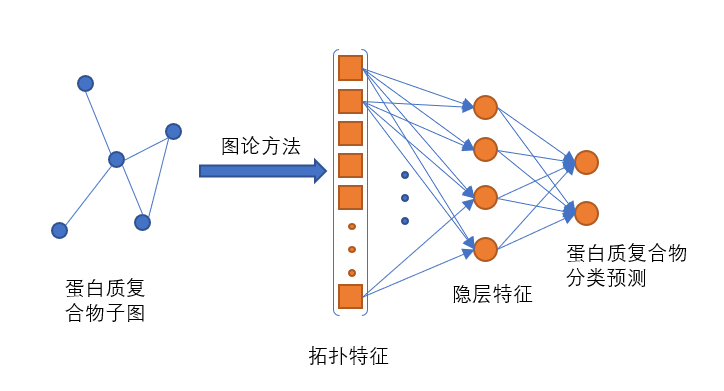
\includegraphics[width=12cm]{entropy-classification}
    \caption{基于图拓扑特征的蛋白质复合物分类模型}
    \label{fig:entropy-classification}
\end{figure}


但是蛋白质复合物中,有大部分复合物是小尺度复合物,其蛋白质个数小于5个。此类复合物的拓扑结构结构简单,提取的拓扑特征具有趋同性。随机的子图在结点数较少的情况下可能形成相同的拓扑特征,此时分类模型无法区分子图是否为真正的复合物。

蛋白质复合物网络是一个高维结构,可以通过挖掘蛋白质在网络中所处的位置和其周围相互作用关系挖掘蛋白质的潜在特征表示,将网络的高维数据转换为蛋白质的低维嵌入表示,成为每一个蛋白质初始的特征向量。

在不引入额外的生物学信息的情况下,本文提出了基于结点的全局拓扑特征的复合物局部子图分类模型。该模型仅使用网络的拓扑特征,利用图卷积神经网络在将拓扑信息与局部子图相互融合,最终得到局部子图的总体特征并做相应的分类与回归处理。

\section{基于图卷积神经网络的复合物筛选模型}
\label{section:NodeConv:detail}

本节分别介绍基于结点卷积单层更新的具体实现,以及基于该单层更新方法构建的蛋白质复合物评价模型,最后介绍复合物筛选模型的总体实现流程。

\subsection{基于结点卷积单层更新}
\label{section:NodeConv:single}

本文在\ref{subsection:featPPINetwork:nodeFeatConstruct}部分简单介绍了图卷积神经网络。本节介绍在基于图卷积神经网络的复合物筛选模型中单一图卷积网络的计算方法。

在单一的卷积层中,结点特征的计算方法如下图所示。

\begin{figure}[htbp]
    \centering
    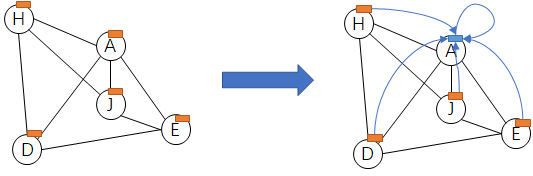
\includegraphics[width=10cm]{GCN/nodeupdate}
    \caption{结点更新过程中数据流程示意图}
    \label{fig:GCN/nodeupdate}
\end{figure}
如图中所示,结点A的特征将有结点$\{A,D,E,H,J\}$共同确定,图中左侧为未更新状态,右侧为更新结点特征过程中的数据流动。其具体过程可以表示为如下的公式。
\begin{equation}
    \label{equ:normalgcn}
    h_i^{(l+1)} = \sigma(b^{(l)} + \sum_{j\in\mathcal{N}(i)}\frac{1}{c_{ij}}h_j^{(l)}W^{(l)})
\end{equation}
其中$\mathcal{N}(i)$表示结点i的所有邻居,${c_{ij}}$表示结点i和结点j度乘积的平方根,其具体计算为$c_{ij} = \sqrt{|\mathcal{N}(i)|}\sqrt{|\mathcal{N}(j)|}$,$\sigma$表示激活函数,$b^{(l)}$表示卷积过程中的偏移值。

在模型中,偏移值设置为0,激活函数为LeakyRelu函数。而在卷积过程中,为了保持结点特征的连续性,每一个子图的结点均添加一条自环,从式中可以得出,添加自环之后,结点特征更新过程中会有一部分信息由自身提供,本模型中平衡系数${c_{ij}}$设置为1。

上式为单个结点的更新过程,将子图中所有结点更新一轮之后即完成一层图卷积过程,图中结点特征从第l层更新到第l+1层。

\subsection{特征子图评价模型}
\label{subsection:NodeConv:flow}

下面从数据流的层面阐述从特征子图数据到样本评价数据的实现流程。基于全局特征的复合物分类模型总体结构如图\ref{fig:GCN/flow}所示。
\begin{figure}[htbp]
    \centering
    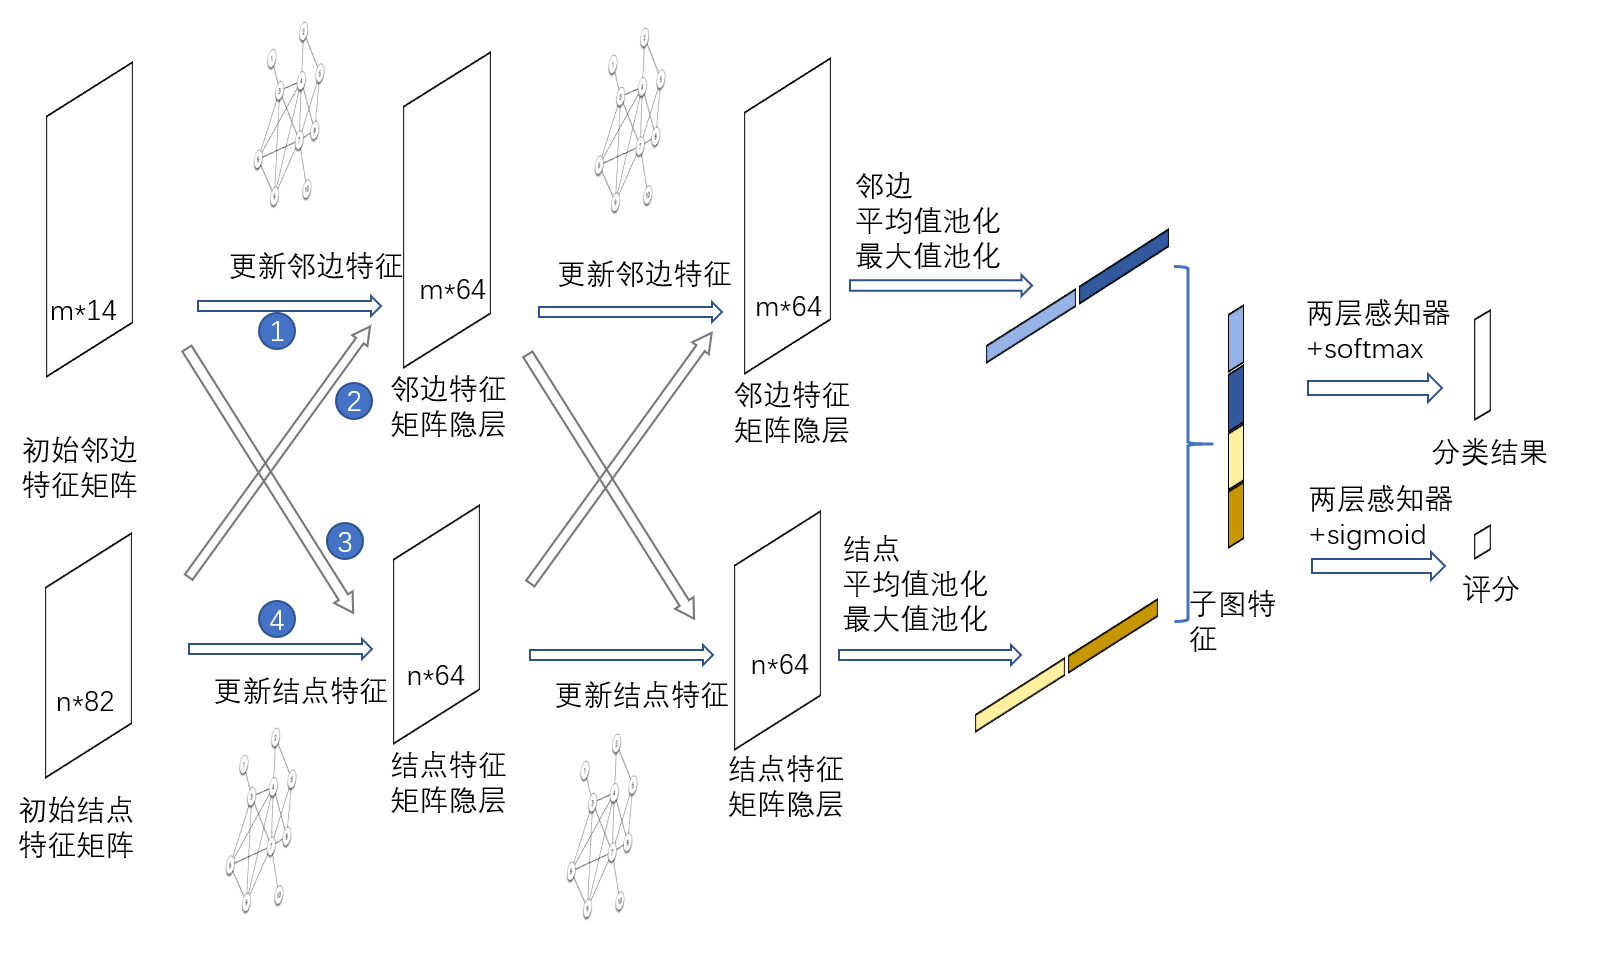
\includegraphics[width=15cm]{GCN/flow}
    \caption{基于图卷积神经网络的复合物筛选模型总体流程}
    \label{fig:GCN/flow}
\end{figure}
模型的初始输入特征结点特征,维度为80维,其中包括基于Deepwalk嵌入特征64维和GAE嵌入特征16维。
在初始特征之后加入了两层图卷积模型,图卷积模型如\ref{section:NodeConv:detail}所示,图卷积可以融合图中结点特征和拓扑结构对结点特征进行更新。图卷积过程中隐层维度设置为64维。两层图卷积之后,采用了对结点特征MaxPooling和MeanPooling的池化方法。两种池化方法的结果进行拼接之后,形成的128维的特征代表图整体特征,如图中1和2部分所示,1部分代表MaxPooling得到的64维特征,2部分代表通过MeanPooling得到的64维特征。

分类与评分部分,1和2两种Pool方法拼接作为代表子图的特征向量。
后续分别为两层感知器和softmax层得到图的分类预测,两层感知器和sigmoid层得到图的评分预测。而两项预测结果采用公式\ref{equ:loss}的损失函数统一起来。通过不断的优化损失函数,可以使得特征向量同时具备分类与评分特征。

分类指标和评分将作为蛋白质复合物的综合评价指标,具体计算方法如\ref{section:NodeConv:allExperienceDesign}中损失函数计算部分所示。

\subsection{筛选模型算法}

本节介绍基于图卷积神经网络的复合物筛选模型的具体算法,包括数据处理,模型训练,样本筛选与结果比对。
具体如算法\ref{alg:nodegcn-screen}所示。

\begin{algorithm}[h]
    \caption{Protein complex screening model based on node convolution} % 名称
    \label{alg:nodegcn-screen}
    \begin{algorithmic}[1]
        \Require
        $Com_t$: train protein complexes;
        $Com_b$: protein complexes before screen;
        $Com_g$: golden bench protein complexes;
        $G$: protein-protein interaction network
        \Ensure
        $F1_a,F1_b/SPA_a,SPA_b$: predicted protein complexes F1/SPA metrix after and before screen;
        \State $n$:PIN node number;$Com_a=None$;
        \State $F_{GAE} \in \mathbb{R}^{n\times 16}=GAE(G)$:compute node feat by GAE algorithm;
        % \ref{subsection:featPPINetwork:nodeFeatConstruct};
        \State $F_{Deepwalk} \in \mathbb{R}^{n\times 64}=Deepwalk(G)$:compute node feat by Deepwalk;algorithm;
        \State $F_{Node} \in \mathbb{R}^{n\times 80}=Concat(F_{GAE},F_{Deepwalk})$;
        \State $Subs_t=Ext(G,F_{Node},Com_t)$: feated subgraph extract algorithm, see in \ref{section:featSubNetworkConstruct:allSample};
        \For{i=0;i<epoch;i++}
        \For{$BSub_t \in Sub_t$} $loss=0$;
        \For{$Sub_t \in BSub_t$}
        \State $Sub_t=NodeConv_0(Sub_t)$;
        \State $Sub_t=NodeConv_1(Sub_t)$;
        \State $F_t=Concat(Maxp(Sub_t),Meanp(Sub_t)),\mathbb{R}^{n_{sub}\times 128}$;
        \State $PredC_t=MLP_C(F_t)$;$PredS_t=MLP_S(F_t)$;
        \State $loss+=\{CEL(PredC_t,LabelC_t)+\alpha \cdot BCEL(PredS_t,LabelS_t)\}$
        \EndFor; optimization $Adam(loss)$;
        \EndFor
        \EndFor
        \State $Subs_b=Ext(G,F_{Node},Com_b)$: feated subgraph extract algorithm, see in \ref{section:featSubNetworkConstruct:allSample};
        \For{$Sub_b \in Subs_b$} $PredC_b=MLP_C(F_b)$;$PredS_b=MLP_S(F_b)$;
        \State $Com_a+=Complex(Sub_b)~if~PredC_b=positive|PredS_b>=0.25$;
        \EndFor
        \State $F1_a=F1(Com_a,Com_g),F1_b=F1(Com_b,Com_g)$;
        \State $SPA_a=SPA(Com_a,Com_g),SPA_b=SPA(Com_b,Com_g)$;
    \end{algorithmic}
\end{algorithm}
模型算法中输入数据包括本文\ref{section:featSubNetworkConstruct:allSample}节构造的训练数据集$Com_t$、待筛选数据集$Com_b$以及蛋白质相互作用网络图结构数据,其中训练数据集由蛋白质复合物的正样本数据集,中间样本数据集和负样本数据集构成,训练数据集中每一个蛋白质符合物样本均具有分类标注与评分标注。

模型的输出数据为待筛选数据集筛选之前的所有样本$Com_b$与筛选之后剩余样本$Com_a$的评价指标,评价指标需要参照真实复合物样本集$Com_g$计算,计算的指标包括F1值和综合评价指标SPA。最终的输出为筛选后F1评价指标$F1_a$、筛选前F1评价指标、筛选后SPA评价指标$SPA_a$、筛选前SPA评价指标$SPA_b$,如算法中输出部分所示。

算法中第2行代表采用图自编码器方法对蛋白质相互作用网络中每一个结点进行编码,得到编码结果为结点特征矩阵$\mathbb{R}^{n\times 16}$,其中n代表互作网络中结点的数量。第3行代表采用深度随机游走获取的结点特征矩阵$\mathbb{R}^{n\times 64}$。通过$Concat$的方法将GAE特征和Deepwalk特征拼接到一起,得到80维的特征矩阵$\mathbb{R}^{n\times 80}$,如第4行所示。算法中第5行和第17行表示结合互作网络,特征数据和蛋白质复合物中的蛋白质集合提取取蛋白质复合物特征子图的方法,其中$Subs_t$表示训练数据集提取的所有特征子图,$Subs_b$为待筛选数据集提取的所有特征子图,其具体实现如\ref{section:featSubNetworkConstruct:allSample}所示。

第6行至第16行表示基于图卷积神经网络的蛋白质评价模型的训练过程,模型采用分批次的训练方法,同一个批次的若干子图训练损失加和作为整个批次的损失,并进行批次更新参数,如第13行和14行所示。算法中第9行和第10行表示两层基于结点的图卷积过程,该过程具体的更新方式如\ref{section:NodeConv:single}所示,模型实现细节已有阐述。第11行表示图读出过程,图读出采用所有结点隐层特征的最大池化$Maxp$和平均池化$Meanp$拼接$Concat$作为子图的特征,其特征维度维$\mathbb{R}^{n_{sub}\times 128}$,其中$n_{sub}$代表该特征子图中的结点数量。第12行表示以子图特征为基础,经过两层分类感知器得到子图的分类结果,分类结果为$\mathbb{R}^{1\times 4}$的矩阵,其和为1,每一个数据表示子图输出对应类别的概率;经过两层回归感知器得到子图的评分结果,评分数据为0至1,代表样本为真实复合物的概率值。第14行表示某一个复合物样本的训练损失,分为分类损失和回归损失,其中有损失平衡系数$\alpha$。

第18行至第22行为模型筛选以及评价阶段。第18行表示对于待筛选复合物$Subs_b$中的每一个特征子图样本,由已经过训练的复合物评价模型得出对应待筛选样本的分类数据和评分数据。在筛选阶段,如果该样本被模型分类为真样本或者其评分高于0.25,则将该样本归类为高评分复合物,添加到筛选结果中$Com_a$,如算法中第19行所示。最终第21行表示筛选后与筛选前复合物样本分别与标准复合物做比对,并分别得出其F1值评价指标,第22行对应SPA值评价指标。评价指标的具体计算如\ref{section:NodeConv:allExperienceDesign}部分所示。

\section{实验参数与评价指标}
\label{section:NodeConv:allExperienceDesign}
本节介绍实验相关环境、实验通用超参数设置、相关优化器以及评价指标,该部分内容适用于本文所有复合物筛选模型的实验,后续章节中不做重复阐述。

\subsection{实验环境}
\label{subsection:allExperienceDesign:Environment}

本文的实验基于Linux系统Ubuntu16.04版本,处理器型号为Intel(R) Xeon(R) CPU E5-2680 v4 @ 2.40GHz,内存大小为128GB。本文代码基于Python编写,其中深度学习框架基于Pytorch,图神经网络框架基于DGL库\cite{wang_deep_2020}。

\subsection{实验参数}
\label{subsection:allExperienceDesign:nums}

由于训练数据的不平衡性,训练模型之前,数据进行了重采样处理,保持各分类训练样本相等。按照$8:2$的比率分割各分类样本,形成训练集和测试集。在分类模型的训练过程中,观察训练集和测试集的损失函数,根据早停策略得到未过拟合最佳模型。
由于各项特征数据存在不平衡性,部分数据如蛋白质长度等数值过大,本文将所有的特征数据进行了统一的归一化和标准化处理。

本文采用0.001的学习率,batch大小设置为32,隐层维度为64,模型使用了两层的GCN网络以及两层的分类器。
采用LeakyRelu作为激活函数和AdamOptimizer作为模型优化器。LeakyRelu激活函数如图\ref{fig:leakyrelu}所示。

\begin{figure}[htbp]
    \centering
    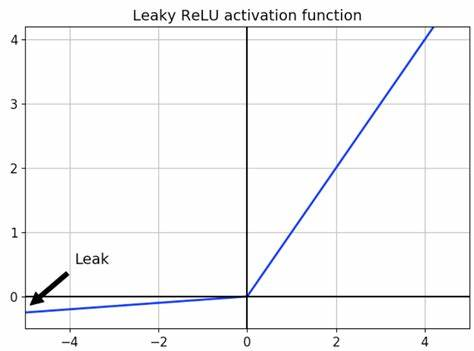
\includegraphics[width=5cm]{leakyrelu}
    \caption{Leaky-Relu 激活函数示意图}
    \label{fig:leakyrelu}
\end{figure}
LeakyRelu激活函数会保留所有为正值的数据,相较于Relu激活函数将所有输入的负值以0输出,LeakyRelu会保留一定的负值输出。


每一个训练复合物样本都具有复合物类别以及相似性评分两项数据,针对这两项属性,本文实验中分别设置了两项损失函数,使用交叉熵损失(Cross Entropy Loss)计算复合物类别分类损失,使用BCE损失(Binary Cross Entropy Loss)计算复合物得分回归损失。由于两项损失在数值上的差异,设置了相应的损失平衡系数。具体损失计算如下所示。
\begin{equation}
    \label{equ:loss}
    loss=CELoss(PL,TL)+\alpha \cdot BCELoss(PS,TS)
\end{equation}
其中,$PL$为预测类别,$TL$为真实类别,$PS$为预测评分,$TS$为真实评分,$\alpha$为损失平衡系数。

\subsection{评价指标}
\label{subsection:allExperienceDesign:metrix}

模型测试阶段,本文将复合物生成算法A在$PIN$网络中运行得到算法A预测的复合物$Complexes_A$,用复合物分类模型筛选所有预测结果,其中如果预测样本在筛选模型中被分类为真样本或者评分高于0.25时,预测样本即可通过筛选。最后所有通过筛选的复合物形成复合物集合$Complexes_A'$。最后使用F1值和PPV指标评估$Complexes_A$和$Complexes_A'$的复合物质量。
评价复合物预测结果的常用指标为精准率(precision)、召回率(recall)和F1值(F1-score)。预测复合物和标准复合物计算邻居相似性(NA-similarity)\ref{equ:compComplexSim:NA}。

按照一般性标准,邻居相似性大于0.25时,预测复合物和标准复合物具有匹配性,表示复合物预测成功。
精准率计算如公式\ref{equ:precision}所示。
其中$PC$为预测复合物集合,$M_{PC}$为预测复合物中具有匹配性的所有复合物集合。精准率表示预测复合物中,预测成功的样本所占比重,衡量预测结果的“查准率”。
召回率段计算如公式\ref{equ:recall}所示。
其中$BC$为标准复合物集合,$M_{BC}$为标准复合物中被预测复合物匹配的集合。召回率表示标准复合物中,能被预测复合物匹配的样本所占的比重,衡量预测结果的“查全率”。
F1值综合考虑查准率和查全率,计算如公式\ref{equ:f1}所示。
从定义看出,当查准率和查全率中有一项指标偏小时,F1值就会偏小。
\begin{equation}
    \label{equ:precision}
    precision=\frac{\left\lvert M_{PC}\right\rvert }{\left\lvert PC\right\rvert }
\end{equation}
\begin{equation}
    \label{equ:recall}
    recall=\frac{\left\lvert M_{BC}\right\rvert }{\left\lvert BC\right\rvert }
\end{equation}
\begin{equation}
    \label{equ:f1}
    f-score=\frac{2\times precision\times recall}{precision + recall }
\end{equation}

除此之外,研究者还提出了多种评价复合物预测质量的指标\cite{shi_protein_2011},包括Sn值、PPV值(Cluster-wise Positive Predictive Value)和Acc值等等。

Sn值具体计算方式图式\ref{equ:Sn}所示,
\begin{equation}
    \label{equ:Sn}
    S_n=\frac{\sum_{i = 1}^{n} \max_{j=1}^{m} t_{ij}}{\sum_{i = 1}^{n}n_i}
\end{equation}
其中${j| 1,2,\dots,m }$表示所有的预测复合物,${i| 1,2,\dots,n }$表示所有的标准复合物,$t_{ij}$表示两个复合物$i,j$之间共同蛋白质的数量,$n_i$表示真实复合物中蛋白质的个数。$S_n$值可以反应真实复合物中蛋白质分子被匹配到个数的平均值。

PPV值具体计算方式如式\ref{equ:PPV}所示,
\begin{equation}
    \label{equ:PPV}
    PPV=\frac{\sum_{j = 1}^{m} \max_{i=1}^{n} t_{ij}}{\sum_{i = 1}^{n} \sum_{j = 1}^{m}   t_{ij}}
\end{equation}
可以看出PPV值反应了预测的复合物的匹配程度,PPV值越高,表示预测复合物和标准复合物的平均重合度越高。

Acc值综合考虑了Sn值和PPV值的结果,能更全面的反应预测复合物集合的质量,其具体计算方法如式\ref{equ:Acc}所示。通常情况下,可以将Sn值、PPV值和Acc值的和作为综合的衡量指标\ref{equ:SPA}。
\begin{equation}
    \label{equ:Acc}
    Acc=\sqrt{S_n\times PPV}
\end{equation}

\begin{equation}
    \label{equ:SPA}
    SPA= Sn+PPV+Acc
\end{equation}

\section{实验设计及结果分析}
\label{section:NodeConv:experience}

本章提出了基于全局特征的复合物筛选模型,该模型使用蛋白质网络得到蛋白质编码,在复合物子图中使用GCN网络将蛋白质编码和子图拓扑结构进行融合。
该模型未引入额外的生物学信息,为了验证模型的有效性,本文进行了如下的对比试验。

第一个对比的模型是使用随机特征GCN图分类模型,子图GCN网络输入的结点特征为随机数据,通过该模型的对比验证全局特征的有效性。

第二个对比的模型是采用图论拓扑统计特征的分类模型\ref{fig:entropy-classification}。计算若干维度的图拓扑特征并进行标准化处理,作为子图特征的代表,用于后续多层感知器分类模型的输入。具体特征提取拓扑特征如表\ref{tab:datasets:statisticgraphfeat}所示。

\begin{table}[h]
    \centering
    \caption{图拓扑特征统计}
    \label{tab:datasets:statisticgraphfeat}
    \begin{tabular}{C{3cm}C{2cm}L{8cm}}
        \toprule
        \textbf{拓扑特征类型} & \textbf{维数} & \textbf{具体描述}                \\
        \midrule
        图总体特征            & 2             & 图结点数,图密度                 \\
        度分布特征            & 4             & 度数平均值、最大值、最小值、方差 \\
        聚类系数特征          & 3             & 聚类系数最大值、平均值、方差     \\
        其他特征              & 1             & 度同配型(degree assortativity) \\
        \bottomrule
    \end{tabular}
\end{table}

\subparagraph*{实验方案(一)} 稀疏网络中基于图卷积神经网络筛选模型实验

在本文介绍的四个$PPI$网络中,DIP网络的密度最低,为0.0014,其平均度数最低6.98,具有一定的稀疏性。且DIP网络的结点数量较多,为4928个,仅次于Biogrid网络,数据完整性较高。因此方案(一)选择DIP网络作为稀疏网络进行相关实验。

\begin{figure}[htbp]
    \centering
    \subcaptionbox{F1值对比}{\label{fig:result/DIP/F1/node}
        \includegraphics[width=10cm]{result/DIP/F1/node}}
    \vskip0.2cm
    \subcaptionbox{SPA值对比}{\label{fig:result/DIP/SPA/node}
        \includegraphics[width=10cm]{result/DIP/SPA/node}}
    \caption{DIP网络不同模型处理后结果对比}
    \label{fig:result/DIP/node}
\end{figure}

\begin{table}[h]
    \centering
    \caption{DIP网络不同模型处理后结果对比数据}
    \begin{tabular}{C{2cm}C{2cm}C{2cm}C{2cm}C{2cm}}
        \toprule
        \textbf{F1值} & \textbf{原始数据} & \textbf{随机GCN筛选} & \textbf{拓扑方法筛选} & \textbf{全局特征GCN筛选} \\
        \midrule
        Dpclus算法    & 0.414             & 0.352                & 0.328                 & 0.434                    \\
        Clique算法    & 0.296             & 0.222                & 0.238                 & 0.477                    \\
        IPCA算法      & 0.291             & 0.300                & 0.310                 & 0.336                    \\
        \bottomrule
    \end{tabular}
    \begin{tabular}{C{2cm}C{2cm}C{2cm}C{2cm}C{2cm}}
        \toprule
        \textbf{SPA值} & \textbf{原始数据} & \textbf{随机GCN筛选} & \textbf{拓扑方法筛选} & \textbf{全局特征GCN筛选} \\
        \midrule
        Dpclus算法     & 1.333             & 1.340                & 1.330                 & 1.424                    \\
        Clique算法     & 0.658             & 0.596                & 0.656                 & 0.815                    \\
        IPCA算法       & 0.794             & 0.729                & 0.744                 & 0.922                    \\
        \bottomrule
    \end{tabular}
    \label{tab:result/DIP/node}
\end{table}


本文在DIP网络中提取了训练特征子图,其组成为正样本特征子图371个,A类中间样本179个,B类中间样本345个以及负样本764个,其具体的构造方法如\ref{section:featSubNetworkConstruct:allSample}所示。接下来在DIP网络中运行Dpclus算法、Clique算法和IPCA算法,分别得到了预测的蛋白质复合物结果,分别为1178、3224和840个样本,接下来分别构造了特征子图,最终形成了三个待筛选特征子图样本数据集。

实验中在训练特征子图数据集基础上训练了基于图卷积神经网络的评价模型。模型训练完成之后,分别对三个待筛选特征子图样本数据集中的样本进行了测试将其中符合要求的复合物保留下来,作为筛选后样本数据集。接下来分别对比了筛选前后样本数据集F1值和综合评价指标。

按照以上的实验方法本章对比了基于随机结点特征模型和基于图论拓扑特征的模型,随机结点特征的对比可以确定嵌入结点特征的有效性,基于图论拓扑特征的模型作为拓扑特征的Base模型,总体的实验结果如下所示。



图\ref{fig:result/DIP/node}为在DIP网络中,随机结点特征模型、图论拓扑特征模型以及全局特征模型筛选之后结果的对比,包含了F1值对比图和SPA值对比图。表\ref{tab:result/DIP/node}为实验结果具体数据。

\subparagraph*{实验方案(二)} 稠密网络中基于图卷积神经网络筛选模型实验

在本文介绍的四个$PPI$网络中,Biogrid网络的密度最高,为0.0038,其平均度数最低21.40,远高于其他$PPI$网络,相较于其他网络Biogrid网络稠密性较高。且Biogrid网络的具有最高的结点数量,数据为5573。因此方案(二)选择Biogrid网络作为稠密网络进行相关实验。

\begin{figure}[htbp]
    \centering
    \subcaptionbox{F1值对比}{\label{fig:result/Biogrid/F1/node}
        \includegraphics[width=10cm]{result/Biogrid/F1/node}}
    \vskip0.2cm
    \subcaptionbox{SPA值对比}{\label{fig:result/Biogrid/SPA/node}
        \includegraphics[width=10cm]{result/Biogrid/SPA/node}}
    \caption{Biogrid网络不同模型处理后结果对比}
    \label{fig:result/Biogrid/node}
\end{figure}

\begin{table}[h]
    \centering
    \caption{Biogrid网络不同模型处理后结果对比数据}
    \begin{tabular}{C{2cm}C{2cm}C{2cm}C{2cm}C{2cm}}
        \toprule
        \textbf{F1值} & \textbf{原始数据} & \textbf{随机GCN筛选} & \textbf{拓扑方法筛选} & \textbf{全局特征GCN筛选} \\
        \midrule
        Dpclus算法    & 0.425             & 0.444                & 0.254                 & 0.470                    \\
        Clique算法    & 0.202             & 0.216                & 0.196                 & 0.372                    \\
        IPCA算法      & 0.293             & 0.123                & 0.331                 & 0.365                    \\
        \bottomrule
    \end{tabular}
    \begin{tabular}{C{2cm}C{2cm}C{2cm}C{2cm}C{2cm}}
        \toprule
        \textbf{SPA值} & \textbf{原始数据} & \textbf{随机GCN筛选} & \textbf{拓扑方法筛选} & \textbf{全局特征GCN筛选} \\
        \midrule
        Dpclus算法     & 1.796             & 1.187                & 1.382                 & 1.871                    \\
        Clique算法     & 0.901             & 0.532                & 0.675                 & 1.009                    \\
        IPCA算法       & 0.859             & 0.886                & 0.810                 & 0.970                    \\
        \bottomrule
    \end{tabular}
    \label{tab:result/Biogrid/node}
\end{table}



本文在Biogrid网络中提取了训练特征子图,其组成为正样本特征子图621个,A类中间样本192个,B类中间样本975个以及负样本819个,其具体的构造方法如\ref{section:featSubNetworkConstruct:allSample}所示。接下来在DIP网络中运行Dpclus算法、Clique算法和IPCA算法,分别得到了预测的蛋白质复合物结果,分别为1078、6250和438个样本,接下来分别构造了特征子图,最终形成了三个待筛选特征子图样本数据集。
后续其他具体实验细节如方案(一)。



图\ref{fig:result/Biogrid/node}为在Biogrid网络中,随机结点特征模型、图论拓扑特征模型以及全局特征模型筛选之后结果的对比,包含了F1值对比图和SPA值对比图。表\ref{tab:result/Biogrid/node}为实验结果具体数据。


\subparagraph*{实验结论} ~

实验方案(一)中图\ref{fig:result/DIP/node}显示在DIP网络中随机GCN筛选和基于拓扑GCN筛选可能导致F1值的降低和评价指标的降低,原因为简单模型在学习的过程中会直接学习直观的拓扑关系,导致分类的错误率较高,在筛选过程中会错误的剔除正样本,导致筛选之后样本质量反而降低。
实验方案(二)中图\ref{fig:result/Biogrid/node}显示全局特征的GCN筛选对Clique算法的提升十分显著,Clique算法是一种基于3-clique结构挖掘复合物的算法,该算法是一种基于密集连边发现复合物的算法,在Biogrid网络中,网络密度相较于DIP网络高了5.2,因此在Biogrid网络中,Clique算法会相应的产生更多的样本,从而为算法优化提供空间。

基于全局拓扑数据结点嵌入的复合物筛选模型,在稀疏网络和密集网络中对比的无特征方法、局部拓扑特征方法中均取得了最佳的F1值和SPA值,证明了结点嵌入的复合物筛选模型的有效性。

\section{本章小结}
\label{section:NodeConv:summary}

本章基于拓扑结构出发,提出了基于全局拓扑数据嵌入的复合物筛选模型,通过GAE和Deepwalk嵌入结点特征,基于图卷积神经网络的蛋白质复合物子图评分模型将结点特征融合。本章详细阐述了单层卷积过程以及整体模型的结构与算法流程。同时本章介绍了通用性的实验环境、实验参数以及评价指标。最后本章在子图拓扑特征模型,无嵌入图卷积模型并进行了相关实验,实验结果表明了结点嵌入特征和筛选模型的有效性。
